\chapter[Informações Gerais]{Informações Gerais}
\label{chap:informacoesGerais}
	
	Nesta seção serão abordados tópicos introdutórios aos desenvolvimento deste documento. Para isso, são apresentandos nos subtópicos a seguir as informações no qual expressam a ideia do projeto inicialmente.

	\section[Integrantes do Grupo]{\emph{Integrantes do Grupo}}
	\label{sec:informacoesGerais_integrantes}

		O grupo é composto por 6 colaboradores e por 1 gestor. A seguir são apresentados os nomes e suas respectivas matriculas.

		\label{subsubsec:informacoesGerais_integrantes_tables}
		\begin{table}[h]
			\centering 
			\begin{tabular}{r|c}

				Nome do Integrante & Matricula \\
				
				\hline

				Augusto Samuel Modesto & 12/0111314 \\
				Matheus Coelho & 12/0129345 \\
				Paulo Ananias de Sousa & 12/0131919 \\
				Renner Parente Magalhães & 13/0132101 \\
				Ruan Kevelin Neves & 12/0021978 \\
				Samantha de Oliveira Gil & 12/0135175 \\
				Willian Ricardo Coelho & 14/0166033 \\

			\end{tabular}
			\caption[Tabela de Integrantes do Grupo]{Tabela de Integrantes do Grupo.}
			\label{tab:informacoesGerais_integrantes_.tables}
		\end{table}

		Para a escolha do gestor, fora feito uma eleição para a escolha democrática do mesmo. Ao final da eleição, como representante do grupo, o \textbf{Augusto Samuel Modesto} foi elegido como o gestor do grupo.

	\section[Tema do Projeto]{\emph{Tema do Projeto}}
	\label{sec:informacoesGerais_tema}

		Para a escolha do tema, foram analisadas diversas temáticas. Entre as mais importantes estavam:

		\begin{enumerate}
			\item{\textbf{Produção de cerveja} – Produção de cerveja na empresa AMBEV;}
			\item{\textbf{Rede de Fast Food} – Rede de produção de hambúrgueres, milk shakes, entre outros;}
			\item{\textbf{Produção de Latinha de refrigerante} – Produção de latinhas na distribuidora empresa AMBEV.}
		\end{enumerate}

		Levando em consideração a facilidade de informações que podem ser obtidas nas redes de Fast Food, decidiu-se a escolha dela. Então, foram levantadas duas redes diferentes de fast food, o Giraffas e o Bob’s. No entanto, optou-se em escolher o Bob's como empresa a ser estudada. Para definição do escopo para pesquisa foram escolhidas duas franquias em diferentes localidades, neste caso, as franquias no aeroporto e no Taguatinga Shopping. A escolha de diferentes franquias servirá como parâmetro de comparações entre o processo de produção de ambas permitindo assim descrever as diferenças equivalentes as suas divergentes localizações geográficas. Cabe ressaltar que, toda a pesquisa gira em torno da franquia no Taguatinga Shopping, e portanto, a outra franquia entrará apenas para comparativos nos casos em que sejam necessários. 

	\section[Ferramenta de Gestão]{\emph{Ferramenta de Gestão}}
	\label{sec:informacoesGerais_ferramenta}

		Para o controle das atividades, foram analisadas duas ferramentas para gerenciamentos das atividades produzidas pelo grupo. São elas:

		\begin{itemize}
			\item{\textbf{Trello};}
			\item{\textbf{ScrumMe}.}
		\end{itemize}

		Ambas as ferramentas possuim características muito próximas trabalhando com a ideia do \emph{Kanban} promovida pelas metodologias ágeis. Esse método permite uma fácil interação além de possuir uma curva de aprendizagem muito baixa, isso pode ser percebido ao longo da disciplina, uma vez que os integrantes conseguiram trabalhar de forma eficiente na ferramenta escolhida.

		Avaliandos ambas as ferramentas, pode-se perceber que ambas possuiam um bom desempenho para o gerenciamento das atividades em geral. O \textbf{ScrumMe} apresentou uma excelente ferramenta de gráficos, no qual permite-se verificar as atividades dos integrantes do grupo por meio de percentuais de trabalho, sendo possível validar quem trabalhou e quanto trabalhou. No entanto, a ferramenta escolhida foi o \textbf{Trello} por ser muito mais simplista no seu funcionamento do que a outra. Esse critério foi adotado tendo em vista que a equipe de trabalho não possuia experiência em metodologia ágeis. Logo, uma ferramenta que facilitasse a aprendizagem em sua simplidade teria muito mais relevância do que alguns gráficos de desempenho.

		A imagem a seguir ilustra o estado final da ferramenta de gerenciamento tarefas - \textbf{Trello}.
		\newpage
		\begin{figure}[h]
			\centering
			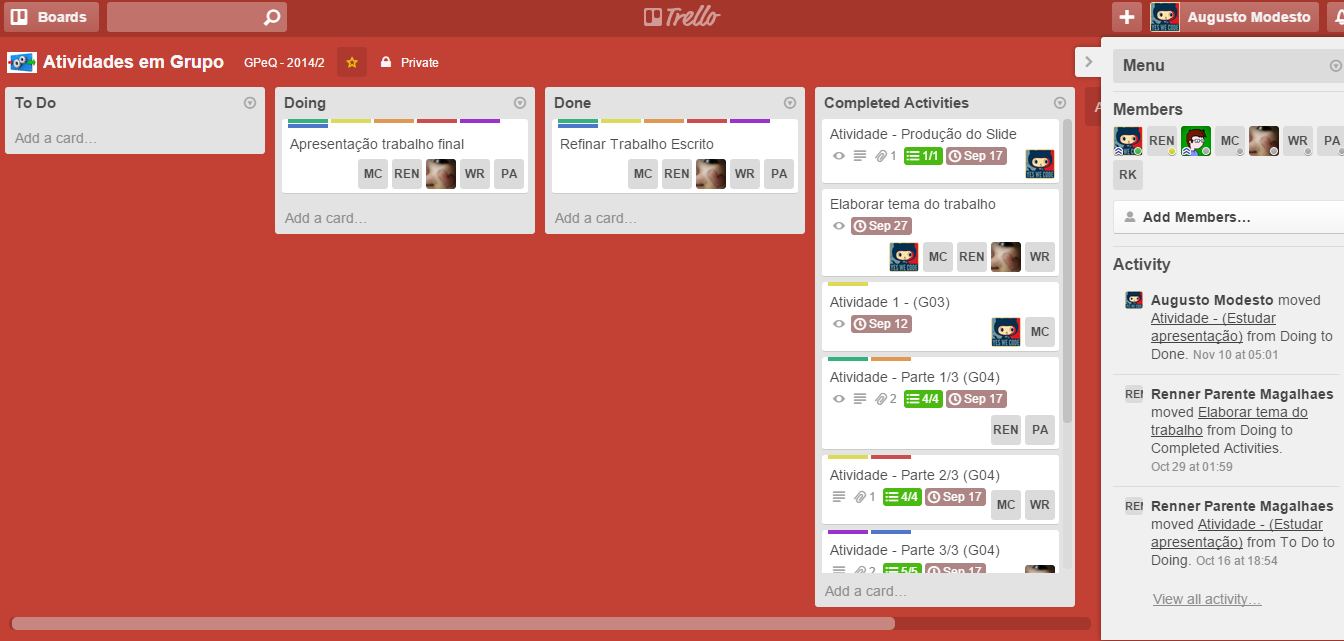
\includegraphics[scale=0.4]{trello}
			\caption[Estado final do Trello após encerramento das atividades]{Estado final do Trello após encerramento das atividades.}
			\label{fig:trello}
		\end{figure}